\documentclass[12pt,a4paper]{report}
\usepackage[utf8]{inputenc}
\usepackage{amsmath}
\usepackage{amsfonts}
\usepackage{amssymb}
\usepackage{graphicx}
\usepackage{enumitem}
\usepackage[left=2cm, right=2cm, top=4cm, bottom=2cm]{geometry}

\begin{document}
	\begin{titlepage}
		\centering
		{\scshape\LARGE Universidad Nacional Autónoma de México \par}
		\vspace{1cm}
		{\scshape\Large Probabilidad I\par}
		\vspace{1.5cm}
		{\huge\bfseries Tarea IV\par}
		\vspace{.5cm}

		{\Large\itshape Alan Ernesto Arteaga Vázquez \par}
		 \vspace{.5cm}
		{\Large\itshape Raúl Llamosas Alvarado \par}
		 \vspace{.5cm}
		{\Large\itshape Edgar Quiroz Castañeda \par}
	    \vspace{.5cm}
		{\Large\itshape Jean Paul Ruiz Melo\par}
		\vspace{.5cm}
		{\Large\itshape Sandra Del Mar Soto Corderi \par}

		\vfill
		 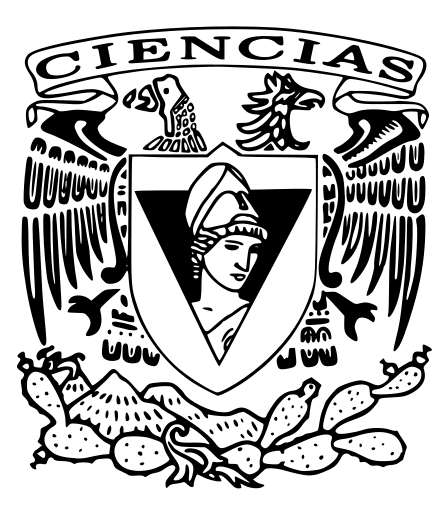
\includegraphics[width=0.5\textwidth]{escudo.png}
		\vfill

		{\large Lunes 15 de octubre del 2018 \par}
	\end{titlepage}

	\pagebreak
	\setlength{\voffset}{-0.75in}
	\setlength{\headsep}{5pt}

	\begin{enumerate}
		%Ejercicio 1
		\item {
			Sea $A$ un evento $(A \in F)$. Definimos $X$ por
			\[
				X(\omega) =
				\begin{cases}
					1, $ si $\omega \in A\\
					0, $ si $\omega \not\in A
				\end{cases}
			\]
			¿Es $X$ variable aleatoria?

			Tenemos que una variable aleatoria está definida como: \\
			\textbf{Definición:} Para un espacio de probabilidad $P=(\Omega,F,P)$ tenemos que $X:\Omega \mapsto \mathds{R}$ es una variable aleatoria si:
        		   	\begin{center}
			   $ \lbrace w\in \Omega : X(w) \leq x \rbrace \in F.$
			\end{center}
			Donde $x\in \mathds{R}$ y $Im^{-1}(X)=(-\infty,x]$. Tenemos que la función está dada para un evento en específico de A. Si F está dado como: \\
			\begin{center}
			    $F= \lbrace A, A_{1},...,A_{n} \rbrace \subset P(\Omega): \Omega = \lbrace O_{1},...,O_{k} \rbrace $
			\end{center}
			Tenemos que los valores de la función está acotada por 1 y por 0. Entonces los rangos de x corren en $(-\infty,0),[0,1),[1,\infty)$. Tenemos entonces que:\\
		    \begin{center}
		        si $x\in (-\infty,0) \Rightarrow \lbrace w \in \Omega: X(w) \leq x \rbrace =  \emptyset  \in F $\\
		        si $x\in [0,1)  \Rightarrow \lbrace w \in \Omega: X(w) \leq x \rbrace = \lbrace w\in \Omega : X(w)=0 \rbrace$
		    \end{center}
		    Pero ésto solamente sucede cuando $w\notin A $, es decir cuando $w \in A^c$, pero como F es una $\sigma-algebra$ entonces claramente $A^c\in F$ por lo que $\lbrace w \in \Omega : X(w) \leq x \rbrace = A^c \in F$ si $x\in [0,1)$.  Ahora tenemos que:\\
		    \begin{center}
		        si $x\in [1,\infty) \Rightarrow \lbrace w \in \Omega : X(w) \leq x \rbrace = \lbrace w \in \Omega : X(w)=1 \rbrace  = \lbrace w\in \Omega: w \in A \rbrace = A$.
		        Y $A \in F$ por hipótesis. Entonces cumple los requisitos de que sea una variable aleatoria$_{\blacksquare}$
\end{center}

		}

		%Ejercicio 2
		\item {
			Considere un espacio de probabilidad $\Omega = \{1, 2, 3, 4, 5, 6\}$ y
			$F = \{\emptyset, \Omega, \{2, 4, 6\}, \{1, 3, 5\}\}$.\\
			Sean $X_1, X_2 : \Omega \rightarrow \mathbb{R}$ definidas como:
			\begin{align*}
				X_1(\omega) &= \omega^2\\
				X_2(\omega) &= \begin{cases}																						1, \omega $ par$\\																			0, \omega $ impar$																			\end{cases}
			\end{align*}
			¿Son $X_1$ y $X_2$ variables aleatorias en este espacio de probabilidad?

			Tenemos que: \\
			\begin{center}
			    $X_{1}(w)= \begin{cases} 1, si\ \omega=1\\ 4,si \ \omega=2 \\ 9, si \ \omega=3\\ 16, si \ \omega=4 \\ 25, si \ \omega=5 \\ 36, si \ \omega=6  \end{cases}$
			\end{center}
			Entonces que los intervalos a considerar son $(-\infty,1),[1,4),[4,9),[9,16),[16,25),[25,36),[36,\infty)$\\
			\begin{center}
			    si $x\in (-\infty,1) \Rightarrow \lbrace w\in \Omega : X(w)\leq x \rbrace = \emptyset \in F $ \\
			    si $x\in [1,4) \Rightarrow \lbrace w \in \Omega : X(w) \leq x \rbrace = \lbrace 1 \rbrace \notin F$
			\end{center}
			Como podemos ver, no se encuentra en F por lo tanto  $X_{1}$ no es una variable aleatoria. Ahora, tenemos que:\\
			\begin{center}
			    $X_{2}(w) = \begin{cases}
			    1, si \ \omega \in \lbrace 2,4,6 \rbrace \\
			    0, si \ \omega \in \lbrace 1,3,5 \rbrace
			    \end{cases}$
			\end{center}

			Los intervalos a considerar son $(-\infty,0),[0,1),[1,\infty)$ entonces:\\
			\begin{center}
			    si $x\in (-\infty,0) \Rightarrow \lbrace w\in \Omega: X(w) \leq x \rbrace = \emptyset \in F. $\\
			    si $x\in [0,1) \Rightarrow \lbrace w \in \Omega: X(w) \leq x \rbrace = \lbrace 1,3,5 \rbrace \in F$  \\
			    si $x\in [1,\infty) \Rightarrow \lbrace w\in \Omega: X(w)\leq x \rbrace = \lbrace 2,4,6 \rbrace \in F$
			\end{center}
Entonces sí es una variable aleatoria. Entonces en conclusión $X_{2}$ es una variable aleatoria pero $X_{1}$ no lo es.\\
		}

		%Ejercicio 3
		\item {
			Sea $f$ una función definida por
			\[
				f(x) = \begin{cases}
								x+1, $ si $ -1 \leq x \leq 0\\
								2x-6, $ si $ 3 \leq x \leq c\\
								0, $ en otro caso$
			\end{cases}
			\]
			Con $c$ constante.
			\begin{enumerate}
				\item{
					Determine el valor de $c$ de tal manera que $f$ sea una función de
					densidad.


					Como es una función de densidad continua tenemos que tiene que cumplir lo siguiente:
					\begin{center}
					    $$\int_{-\infty}^{\infty} f(x) dx = \int_{-\infty}^{-1}f(x)dx+\int_{-1}^{0}f(x)dx+\int_{0}^{3}f(x)dx+\int_{3}^{c}f(x)dx+\int_{c}^{\infty}f(x)dx$$\\
					    $$=0+\int_{-1}^{0}(x+1)dx+0+\int_{3}^{c}(2x+6)dx+0=$$\\
					    $$(\frac{x^2}{2}+x)|_{-1}^{0}+2[(\frac{x^2}{2}+3x)|_{3}^{c}]=1$$\\
					    $$(\frac{0^2}{2}+0)-(\frac{(-1)^2}{2}-1)+2[(\frac{c^2}{2}+3c)-(\frac{9}{2}+9)]=1$$ \\
					    $$\frac{1}{2}+2[(\frac{c^2+6c}{2})-(\frac{27}{2})]=1$$\\
					    \end{center}
					 Y eso solo sucede cuando:
					\begin{center}
					    $$c^2+6c-27+\frac{1}{2}=1$$\\
					    $$c^2+6c-\frac{55}{2}=0$$
					\end{center}
					Cuyos valores que resuelven dicha ecuación son:\\
					\begin{center}
					    $c_{1}=\frac{-6+\sqrt{36+110}}{2}=\frac{-6+\sqrt{146}}{2}$\\
					    $c_{2}=\frac{-6-\sqrt{146}}{2}$
					\end{center}
					Tenemos que el valor tendría que ser positivo para que ésto tuviese sentido y dado que $c_{1}\approx 3.041 $ se tiene que éste será el valor que tenga que tomar c. Entonces el valor de c es:
					\begin{center}
					   $$ c=\frac{-6+\sqrt{146}}{2}$$
					\end{center}
				    }

				\item {
					Encuentre la función de distribución correspondiente a $f$.\\ \\
					Al tratarse de una función continua se tiene que $F(x)= \int_{-\infty}^{x} f(t)dt$ entonces se sigue que:\\
					\begin{center}
					    $F(x)= \begin{cases}
					    \frac{x^2}{2}+x, \ $si$ \ -1\leq x \leq 0 \\
					    \frac{3x^2}{2}-5x, \ $si$ \ 3\leq x \leq  \frac{-6+\sqrt{146}}{2}

					    \end{cases}$
					\end{center}
					Ya que que al tratarse de una función acumulativa se suma a la integral  $\int 2x-6$ la integral $\int x+1$ debido a que es acumulativa.
				}
\end{enumerate}
		}

		%Ejercicio 4
		\item {
			Sea $f$ una función definida por
			\[
				f(x) = \begin{cases}
								cr^x, $ si $ x \in \{0, 1, ...\}\\
								0, $ en otro caso$
							 \end{cases}
			\]
			En donde $0 < r < 1$. Encuentre $c$ para que $f$ sea función de densidad.\\
			Podemos notar que es una funcion de densidad discreta, entonces tenemos:
			\begin{center}
			    $1 = \sum_{x=0}^{\infty} P(i)$
		    \end{center}
		    Donde $P(i) = cr^{x}$. Entoces sustituyendo tenemos:
		    \[1 = \sum_{x=0}^{\infty} cr^{x}\]
		    \[1 = c\sum_{x=0}^{\infty} r^{x}\]
		    \[\frac{1}{c} = \sum_{x=0}^{\infty} r^{x}\]
		    Entonces esto es la serie geométrica:
		    \[\frac{1}{c} = 1 + r + r^{2} + r^{3} + ...\]
		    Y como r es un fración, converge a:
		    \[\frac{1}{c} = \frac{1}{1-r}\]
		    Entonces para que $f$ sea función de densidad:
		    \[c = r-1\]
		}

		%Ejercicio 5
		\item {
		La función de densidad de una variable aleatoria $X$ es
		\[f_X(x) = \gamma x^2 e^{-kx}\mathbb{I}_{(0, \infty)}\]
		Donde $k > 0$.
		\begin{enumerate}
			\item {
				Encontrar el valor de $\gamma$.\\
				Tenemos que:
    			\[1 = \int_{0}^{\infty} \gamma x^2 e^{-kx} dx\]
    			Entonces resolviendo la integral tenemos:
    			\[= \gamma \int x^{2}e^{-kx}\]

    			\[= \gamma (- \frac{x^{2}e^{-kx}}{k} - \int \frac{2xe^{-kx}}{k})\]

    			\[= \gamma (- \frac{x^{2}e^{-kx}}{k} + \frac{2}{k}(-\frac{xe^{-kx}}{k}- \int -
    				\frac{e^{-kx}}{k}))\]

    		    \[= \gamma (- \frac{x^{2}e^{-kx}}{k} + \frac{2}{k}(-\frac{xe^{-kx}}{k}- \frac{1}{k^{2}} ( \int e^{u})); u = -kx , dx = \frac{-1}{k}du\]

    			\[= \gamma (- \frac{x^{2}e^{-kx}}{k} + \frac{2}{k}(-\frac{xe^{-kx}}{k}- \frac{e^{-kx}}{k^{2}}))\]

    			\[= \gamma (- \frac{x^{2}e^{-kx}}{k} - \frac{2xe^{-kx}}{k^{2}}- \frac{e^{-kx}}{k^{3}})\]

    			\[ = -\gamma (\frac{(k^{2}x^{2} + 2kx + 2)e^{-kx}}{k^{3}}\Big|_0^\infty \]
    			Resolviendo, tenemo:
    			\[ 1 = \frac{2\gamma}{k^{3}}\]
    			Entonces $\gamma = \frac{k^{3}}{2}$.
			}
			\item {
				Encontrar la función de distribución $F_X$ de la variable aleatoria
				$X$.\\

				Entonces tenemos:
					\[FX(x) = \int_{0}^{x} \gamma x^2 e^{-kx} dx\]
				Pero ya tenemos que $\gamma = \frac{k^{3}}{2}$, entonces:
					\[FX(x) = \int_{0}^{x} \frac{k^{3}}{2} x^2 e^{-kx} dx\]
				Entonces calculando el integral tenemos:
					\[FX(x) =  \frac{(k^{2}x^{2} + 2kx + 2) e^{-kx}}{2}\Big|_0^x \]
				Y sustituyendo tenemos:
					\[FX(x)= \frac{e^{-kx} (2e^{kx} - k^{2} x^{2} -2kx - 2)}{2}\]
			}
			\item {
				Calcule $P(0 < X < \frac{1}{k})$
				Tenemos:
				\[ P(a < X < b) = FX(b) - FX(a)\]
				Entonces:
				\[=P(0 < X < \frac{1}{k}) = FX(\frac{1}{k}) - FX(0)\]
				\[=\frac{e^{-k\frac{1}{k}} (2e^{k\frac{1}{k}} - k^{2} \frac{1}{k}^{2} -2k\frac{1}{k} - 2)}{2} - \frac{e^{-k0} (2e^{k0} - k^{2} 0^{2} -2k0 - 2)}{2}\]
			    \[=\frac{0.367 (5.43 - 5)}{2} - \frac{1 (2 - 2)}{2}\]
				\[0.079 - 0\]
				\[=0.079 \]
			}
		\end{enumerate}
		}

		%Ejercicio 6
		\item {
			Sea
			\[
				f(x) = \begin{cases}
								0, $ si $ x < 0\\
								\frac{1}{2}\beta, $ si $ 0 \leq x < 1\\
								\frac{1}{2}, $ si $ 1 \leq x < 2\\
								\frac{1}{2}(1-\beta), $ si $ 2 < x < 3\\
								0, $ si $ x \geq 3
						 	 \end{cases}
			\]
			Donde $0 < \beta < 1$. Encontrar la función de distribución $F_X$\\

			Si x $<$ 0, se queda en cero.

			Cuando 0 $\leq$ X $<$ 1, tenemos:
		    \[\int_{0}^{x} \frac{1}{2}\beta dx = \frac{\beta x}{2}\]
		    Para 1 $\leq$ X $<$ 1:
		    \[\int_{1}^{x} \frac{1}{2}dx = \frac{(x-1)}{2}\]
		    Usando el anterior tenemos:
		    \[\frac{(x-1)}{2} +  \frac{\beta x}{2} \]
		    Para 2 $\leq$ X $<$ 3:
		     \[\int_{2}^{x}\frac{1}{2}(1-\beta)dx = -\frac{(x-2)x}{4}\]
		     Lo cual es:
		     \[-\frac{(x-2)x}{4} + \frac{(x-1)}{2} +  \frac{\beta x}{2}\]
		     Entonces la función de distribución es:
		     	\[
				f(x) = \begin{cases}
								0, $ si $ x < 0\\
								\frac{\beta x}{2}, $ si $ 0 \leq x < 1\\
								\frac{(x-1)}{2} +  \frac{\beta x}{2}, $ si $ 1 \leq x < 2\\
								-\frac{(x-2)x}{4} + \frac{(x-1)}{2} +  \frac{\beta x}{2}, $ si $ 2 < x < 3\\
								1, $ si $ x \geq 3
						 	 \end{cases}
			\]
		}

		%Ejercicio 7
		\item {
			Demuestre que $f_X(x) = \frac{1}{2}e^{-|x|}\mathbb{I}_\mathbb{R}(x)$ es
			una función de densidad.
		}

			Como la variable aleatoria toma valores continuos, se tiene que para
			demostrar que $f_X^{(x)}$ se trata de una función de densidad, basta con
			probar que:
			\begin{enumerate}
				\item {
					$$f_X^{(x)} \geq 0 \forall x$$

					Veamos el límite de la función cuando $x \rightarrow \infty$, así:
					$$ \lim_{x\to\infty}  \frac{1}{2}e^{-|x|} $$

					(como x tiende a infinito positivo, se sigue:)
					$$ = \lim_{x\to\infty}  \frac{1}{2}e^{-x}
					   = \lim_{x\to\infty}  \frac{1}{2e^{x}} = \frac{1}{\infty} = 0$$

					análogamente, el límite de la función cuando  $x \rightarrow -\infty$:
					$$ \lim_{x\to -\infty}  \frac{1}{2}e^{-|x|} $$

					(como x tiende a infinito negativo, y por la definición de
					valor absoluto, se sigue:)
					$$ = \lim_{x\to -\infty}  \frac{1}{2}e^{-(-x)}
					   = \lim_{x\to -\infty}  \frac{1}{2}e^{x}
					   = \lim_{x\to -\infty}  \frac{e^x}{2}
					   = \frac{1}{2} \lim_{x\to -\infty}  e^x = \frac{1}{2} \cdot 0 = 0$$

					Luego, para cualquier número real, se tiene que $|x|$ es positivo
					para cualquier $x \in \mathbb{R}$, luego, como $e^x$ es positivo
					para cualquier x número real, notemos que:
						$$ 1 = e^0 = e^{-x}e^x $$
					y así:
						$$ e^{-x} = \frac{1}{e^x} $$
					lo cual, resulta ser un número positivo.

					Así, podemos comprobar que $\frac{1}{2}e^{-|x|} = f_X^{(x)} \geq 0 \; \forall x$

				}
				\item {
					$$\int_{-\infty}^{\infty} f_X^{(x)} du = 1$$

					Se tiene que la integral definida de la función $f_X$ viene dada por:
					$$\int_{-\infty}^{\infty} \frac{1}{2}e^{-|x|} dx$$

					lo cual equivale a:
					$$\int_{-\infty}^{0} \frac{1}{2}e^{-|x|} dx +
					  \int_{0}^{\infty} \frac{1}{2}e^{-|x|} dx $$

					luego, como en la primera integral, el intervalo de integración
					es $ -\infty \leq x \leq 0$, y en la segunda $ 0\leq 0 \leq \infty$
					podemos reescribir:
					$$	\int_{-\infty}^{0} \frac{1}{2}e^{-(-x)} dx +
					  	\int_{0}^{\infty} \frac{1}{2}e^{-(x)} dx
					 =  \int_{-\infty}^{0} \frac{1}{2}e^{x} dx +
 					  	\int_{0}^{\infty} \frac{1}{2}e^{-(x)} dx $$

					$$ = \frac{1}{2} \int_{-\infty}^{0} e^{x} dx +
					     \frac{1}{2} \int_{0}^{\infty} e^{-(x)} dx $$

				 	Ahora, considerando que
	 					$$\lim_{x\to \infty}  e^{-x} = \lim_{x\to -\infty} \frac{1}{e^x} = 0$$
	 					$$\lim_{x\to -\infty}  e^x = 0$$
					Tenemos que:
					$$ = \frac{1}{2} [e^0 - e^{-\infty}] -
					     \frac{1}{2} [e^{-{\infty}} - e^{-0}]
					   = \frac{1}{2} [1 - 0] -
   					     \frac{1}{2} [0 - 1] = \frac{1}{2} - (- \frac{1}{2}) = 1 $$
				}
			\end{enumerate}

			Así, como se cumplen $f_X^{(x)} \geq 0 \; \forall x$ y
			$\int_{-\infty}^{\infty} f_X^{(x)} du = 1$, se tiene que $f_X^{(x)}$
			resulta ser una función de densidad de variable aleatoria continua.


		%Ejercicio 8
		\item {
			Sea $X$ una variable aleatoria con función de densidad
				\[f_Y(y) = cy \mathbb{I}_{\{1, 2, 3, 4\}}(y)\]
				\begin{enumerate}
					\item {
						Determinar el valor de $c$ para que $f_Y$ sea una función de
						densidad de probabilidad.

						Como la variable aleatoria $Y$ toma valores discretos,
						se tiene que para que $f_Y$ cumpla ser una funcion de
						densidad de probabilidad debe cumplirse:
							$$ \sum_{j = 1}^{\infty} f_Y^{(y_j)} = 1 $$

						así, se tiene por la definición de $f_Y$ (como para todo
						valor distinto de $1, 2, 3, 4; \; f_Y(y) = 0$):
							$$ 1 = \sum_{j = 1}^{\infty} f_Y^{(y_j)} = 0 + c + 2c + 3c + 4c + 0 + 0 + ... $$
							$$ 1 = \sum_{j = 1}^{\infty} f_Y^{(y_j)} = c + 2c + 3c + 4c $$

						de ahí obtenemos la ecuación:
							$$ 1 = c + 2c + 3c + 4c $$
							$$ 1 = 10c $$
							$$ c = \frac{1}{10} $$

						Así, para que se cumpla $ \sum_{j = 1}^{\infty} f_Y^{(y_j)} = 1 $,
						se sigue que $c$ debe tener el valor $\frac{1}{10}$.
					}
					\item {
						Calcule $P(1 < Y \leq 3)$ y $P(Y < 1 | Y \leq 3)$

						Se tiene que $P(a < y \leq b) = F_Y^{(b)} - F_Y^{(a)}$,
						así, como $Y$ es una variable aleatoria que toma valores
						discretos podemos decir:

						$$ F_Y^{(3)} = \sum_{\{y | y \leq 3 \}} f_Y^{(y)}
						 = f_Y^{(1)} + f_Y^{(2)} + f_Y^{(3)}
						 = \frac{1}{10} + \frac{2}{10} + \frac{3}{10}
						 = \frac{6}{10}$$

						análogamente:
						$$ F_Y^{(1)} = \sum_{\{y | y \leq 1 \}} f_Y^{(y)}
						 = f_Y^{(1)} = \frac{1}{10}$$

						así, se sigue:
						$$ P(1 < Y \leq 3) = F_Y^{(b)} - F_Y^{(a)}
						 = \frac{6}{10} - \frac{1}{10} = \frac{5}{10}$$

						Ahora, para $P(Y < 1 | Y \leq 3)$, se tiene:

						$$ P(Y < 1 | Y \leq 3)
						 = \frac{P[(Y < 1) \cap (Y \leq 3)]}{P(Y \leq 3)}
						 = \frac{P(Y < 1)}{P(Y \leq 3)}$$

						Notemos ahora:
						$$ P(Y \leq 3) = F_Y^{(3)} = \frac{6}{10} $$
						$$ P(Y < 1) = \lim_{h\to 0^+} F_Y^{(1 - h)}
						 = \lim_{h\to 0^+} \sum_{\{y | y \leq 1 - h \}} f_Y^{(y)} $$

						y como la suma se realiza sobre un conjunto vacío, se sigue:

						$$ \lim_{h\to 0^+} \sum_{\{y | y \leq 1 - h \}} f_Y^{(y)} = \lim_{h\to 0^+} 0 = 0 $$

						De esta manera concluimos:
						$$ P(Y < 1 | Y \leq 3) = \frac{P(Y < 1)}{P(Y \leq 3)}
						 = \frac{0}{\frac{6}{10}} = 0 $$
					}
				\end{enumerate}
		}

		%Ejercicio 9
		\item {
			Sea $X$ una variable aleatoria continua con función de densidad
				\[
					f_X(x) = \begin{cases}
										6x(1-x), $ si $ 0 < x < 1\\
										0, $ en otro caso$
									 \end{cases}
				\]
			Calcule $P(|X-\frac{1}{2}| > \frac{1}{4})$.

			Tenemos que la siguiente desigualdad es equivalente a:
			$$ |X-\frac{1}{2}| > \frac{1}{4}
			   = (X-\frac{1}{2} > \frac{1}{4}) \cup (X-\frac{1}{2} < -\frac{1}{4})$$
			$$ = (X > \frac{3}{4}) \cup (X < \frac{1}{4}) $$

			De ahí, podemos reescribir:
				$$ P(|X-\frac{1}{2}| > \frac{1}{4})
				 = P[(X > \frac{3}{4}) \cup (X < \frac{1}{4})]$$

			Luego, como $P$ es una medida de probabilidad, se sigue:
				$$ P[(X > \frac{3}{4}) \cup (X < \frac{1}{4})]
				 = P(X > \frac{3}{4}) + P(X < \frac{1}{4}) $$

			De allí, obtenemos $P(X > \frac{3}{4})$ y $P(X < \frac{1}{4})$, las cuales
			pueden calcularse mediante:
				$$ P(X > \frac{3}{4}) = 1 - P(X \leq \frac{3}{4})
				 = 1 - F_X^{(\frac{3}{4})} $$

			y como $X$ es una variable aleatoria continua, se sigue:
				$$ 1 - F_X^{(\frac{3}{4})} = 1 - \int_{0}^{\frac{3}{4}} 6x(1-x) dx
				   = 1 - [\int_{0}^{\frac{3}{4}} 6x - 6x^2 dx]  $$
				$$ = 1 - [\int_{0}^{\frac{3}{4}} 6x dx - \int_{0}^{\frac{3}{4}} 6x^2 dx ] $$
				$$ = 1 - [3 x^2 \Big|_0^\frac{3}{4} - 2 x^3 \Big|_0^\frac{3}{4}]
				   = 1 - [3 \cdot \frac{9}{16} - 2  \cdot \frac{27}{64} ]
				   = 1 - [\frac{27}{16} - \frac{54}{64} ] $$
				$$ = 1 - [\frac{108}{64} - \frac{54}{64} ]
				   = 1 - [\frac{108}{64} - \frac{54}{64} ]
				   = 1 - [\frac{54}{64}] $$
				$$ = \frac{64}{64} - \frac{54}{64}  = \frac{10}{54} = \frac{5}{32}$$

			Ahora, para $P(X < \frac{1}{4})$:
				$$ P(X < \frac{1}{4}) = \lim_{h\to 0^+} F_Y^{(\frac{1}{4} - h)}
				   =  \lim_{h\to 0^+} \int_{0}^{(\frac{1}{4} - h)} 6x - 6x^2 dx $$
				$$ =  \lim_{h\to 0^+} [3 x^2 \Big|_0^{(\frac{1}{4} - h)} - 2 x^3 \Big|_0^{(\frac{1}{4} - h)}] $$
				$$ =  \lim_{h\to 0^+} [3 (\frac{1}{4} - h)^2 - 2(\frac{1}{4} - h)^3]$$
				$$ =  \lim_{h\to 0^+} [3 (\frac{1}{4} - h)^2 - 2(\frac{1}{4} - h)^3]$$
				$$ =  \lim_{h\to 0^+} [\frac{16h^3+12h^2-9h}{8} + \frac{5}{32}]$$
				$$ =  \frac{16(0)^3+12(0)^2-9(0)}{8} + \frac{5}{32} = \frac{5}{32}$$

			Así, concluimos que :
				$$ P[(X > \frac{3}{4}) \cup (X < \frac{1}{4})]
				 = P(X > \frac{3}{4}) + P(X < \frac{1}{4})
				 = \frac{5}{32} + \frac{5}{32} = \frac{10}{32} = \frac{5}{16}$$
		}

		%Ejercicio 10
		\item {
			Suponga que se selecciona aleatoriamente un punto $z$ del cuadrado con
			esquinas (2, 1), (3, 1), (2, 2,) y (3, 2). Sea $A$ la variable aleatoria
			que mide el área del triángulo con vértices (2, 1), (3, 1) y $z$.\\
			El área de un triángulo es $\frac{b\cdot h}{2}$. \\
			En este caso la base está fija como $b = \sqrt{(2-3)^2+(1-1)^2} = 1$.\\
			Y cómo la base es paralela al eje $x$, ambas entradas son 1,
			entonces la altura del triángulo sería la altura del punto menos la
			altura de la base, o sea $y_z-1, z = (x_z, y_z)$.
			De estas dos cosas, $A = \frac{b \cdot h}{2} = \frac{1 \cdot(y_z-1)}{2}
			= \frac{y_z-1}{2}$
			\begin{enumerate}
				\item {
					¿Cuál es el valor más grande que $A$ puede tomar?\\
					Como la base está fija, el cambio en el área depenede sólo
					de la altura.\\
					Dado el cuadrado, esta altura puede ser a lo más $2-1 = 1$.
					Entonces el área máxima es $A_m = \frac{1\cdot 1}{2} = \frac{1}{2}$.
				}
				\item {
					¿Cuál es el conjunto de puntos para el cuál $A \leq \frac{1}{4}$?
					\begin{align*}
						A &= \frac{y_z-1}{2} \leq \frac{1}{4}\\
						  &\implies y_z-1 \leq \frac{1}{2}\\
						  &\implies y_z \leq \frac{3}{2}
					\end{align*}
					Entonces, ese conjunto de puntos son $\{(x, y) | y \leq \frac{3}{2}\}$
					y están dentro del cuadrado.\\
					Forman una rectángulo dentro del cuadrado con base igual a
					la del cuadrado y altura $\frac{3}{2}$.
				}
				\item {
					Encuentre la función de densidad de $A$.\\
					La densidad es la derivada de la distribución
					\[\frac{d(2x)}{dx} = 2\]
					\[f_X(x) = 2 \mathbb{I}_{[0, \frac{1}{2}]}\]

				}
				\item {
					Encuentre la función de distribución de $A$.\\
					El área no puede ser negativa, ni mayor a $\frac{1}{2}$.
					En otro caso, los puntos que dan un área menor o igual a $k$
					son
					\[A = \frac{y_z-1}{2} \leq k \implies y_z \leq 2k + 1\]
					Que corresponden a todos los puntos dentro del cuadrado y
					debajo de la recta $y = 2k+1$.\\
					Como el área total del cuadrado es 1, y el área de los
					puntos es en rectángulo con base $b = 1$
					y altura $h = 2k+1-1 = 2k$, entonces el área proporcional de
					los puntos es
					$A = \frac{A_{puntos}}{A_{total}} = \frac{1 \cdot 2k}{1} = 2k$
					Entonces, la función de distribución es
					\[F_X(x) = 2x \mathbb{I}_{[0, \frac{1}{2}]}\]
				}
			\end{enumerate}
		}

		%Ejercicio 11
		\item {
			Una póliza de seguros cubre las reclamaciones médicas de los empleados
			de una pequeña compañía.\\
			El valor $V$ de las reclamaciones hechas en un año es descrita mediante
			\[V = 100,000Y\]
			Donde $Y$ es una variable aleatoria con función de densidad
			\[
				f_Y(y) = \begin{cases}
							k(1-y)^4, $ si $ 0 < y < 1\\
							0, $ en otro caso$
						 \end{cases}
			\]
			Donde $k$ es constante. ¿Cuál es la probabilidad de que $V$ exceda 10,000?\\
			Esto sería
			\[V = 100,000Y > 10,000 \implies Y > \frac{1}{10}\]
			Luego, hay que encontrar la distribución
			\begin{align*}
				F_Y(y) &= \int_{-\infty}^{y}{f_Y(u)du} = \int_{0}^{y}{k(1-u)^4du}\\
					   &= k\int_{0}^{y}{(1-u)^4du} = k (\frac{(1-u)^5}{5})\Big|_0^y\\
					   &= k(\frac{(1-y)^5}{5} - \frac{1}{5})
			\end{align*}
			Y tenemos que
			\begin{align*}
				P(Y > \frac{1}{10}) &= 1 - P(Y \leq \frac{1}{10})\\
									&= 1 - F_Y(\frac{1}{10})\\
									&= k(\frac{(1-\frac{1}{10})^5}{5} - \frac{1}{5})\\
									&= k(\frac{59049}{100000} - \frac{20000}{100000})\\
									&= k(\frac{39049}{100000}) = 0.39049k
			\end{align*}
			Entonces, la probabilidad de que $V$ exceda los 10,000 es un poco
			menos del 40\%.
			}

		%Ejercicio 12
		\item {
			Una urna contiene 5 bolas rojas y 5 bolas azules. Se realiza un juego
			que consiste en extraer aleatoriamente 2 bolas de la urna. Suponga que
			si se extraen dos bolas del mismo color, el jugador gana \$1.11 y si se
			extraen dos bolas de distinto color el jugador pierde \$1.00. Si una
			persona participa en el juego dos veces, calcule la probabilidad de que
			la ganancia de esta persona sea mayor a \$0.00.\\
			Nuestro espacio de probabilidad para una ronda dada sería
			$\Omega = \{(c_1, c_2)| c_j \in \{rojo, azul\}\}$.\\
			La probabilidad sería sólo casos favorables sobre totales.
			Los casos totales de una ronda son $10 \cdot 9 = 90$.\\
			Para que las bolas sean del mismo color en una ronda,
			los casos favorables son $10 \cdot 4 = 40$.\\
			Con $M$ el evento de que las bolas tengan el mismo color,
			$P(M) = \frac{40}{90} = \frac{4}{9}$.\\
			Y la probabilidad de que sean de diferente color es
			$P(M^c) = 1 - P(M_i) = \frac{5}{9}$.\\
			Sea $X$ la variable aleatoria que dice cuanto dinero ganas en una
			ronda
			\[
				X(\omega) = \begin{cases}
								1, $ si $ \omega \in M\\
								-1.11, $ en otro caso$
							\end{cases}
			\]
			Para dos rondas, el espacio sería $\Omega^2$.
			Como al inicio de cada participación el estado del juego es el mismo,
			5 bolas de cada color, entonces cada ronda es un experimento
			independiente.\\
			Entonces, la probabilidad de un evento $(A_1, A_2)$ en este espacio es
			$P(A_1 \cap A_2) = P(A_1)P(A_2)$.\\
			La ganancia sería simplemente la suma de la ganancia de las dos rondas.\\
			Entonces, la variable aleatoria $X_2$ que dice cuanto dinero ganas
			en dos rondas sería
			\begin{align*}
				X_2((A_1, A_2)) &= X(A_1)+X(A_2)\\
								&= \begin{cases}
									-1.11-1.11 = -2.22, $ si $ A_1 = A_2 = M^c \\
									1-1.11 = -0.11, $ si $ A_1 = M, A_2 = M^c \\
									-1.11+1 = -0.11, $ si $ A_1 = M^c, A_2 = M \\
									1+1 = 2, $ si $ A_1 = A_2 = M \\
								\end{cases}
			\end{align*}

			Entonces la densidad de $X_2$ sería
			\[
				f_{X_2}(x) = \begin{cases}
							P(M)^2 = \frac{16}{81}, $ si $ x = 2\\
							P(M)P(M^c) + P(M^c)P(M) = \frac{40}{81}, $ si $ x = -0.11\\
							P(M^c)^2 = \frac{25}{81}, $ si $ x = -2.22\\
							0, $ en otro caso$
						 \end{cases}
			\]
			Finalmente,
			\begin{align*}
				P(X_2 > 0) &= 1 - P(X_2 \leq 0) \\
						 &= 1 - \sum_{x \leq 0}{f_{X_2}(x)}\\
						 &= 1 - (f_{X_2}(-2.22)+f_{X_2}(-0.11))\\
						 &= 1 - (\frac{25}{81} + \frac{40}{81})
						 = 1- \frac{65}{81}
						 = \frac{16}{81}\\
						 &\approx 0.2
			\end{align*}
			Entonces la probabilidad de no perder dinero después de dos rondas
			es poco menos de 20\%.

		}

		%Ejercicio 13
		\item {
			Sea $X$ una variable aleatoria con función de densidad dada por
			\[f_X(x) = \frac{1}{2}e^{-|x|}\mathbb{I}_{\mathbb{R}}(x)\]
			Si $Y = X^2$, encuentre la función de distribución acumulada de $Y$.

			Para obtener la función de distribución acumulada usamos la ley de estadística inconsciente y tenemos que:

		$F_{x}(y) = P(Y \leq y) = P(X^2\leq y) = P(-\sqrt{y} \leq X \leq \sqrt{y})$	\\

			Ya que es una variable aleatoria continua, y basándonos en cómo definimos la función de distribución arriba, el resultado sería la siguiente integral:
			$\int_{-\sqrt{y}}^{\sqrt{y}} \frac{1}{2}e^{-|x|}$

			Desarrollamos:
			 \[
               \int_{-\sqrt{y}}^{\sqrt{y}} \frac{1}{2}e^{-|x|}
                =
                 \int_{-\sqrt{y}}^{0} \frac{1}{2}e^{x}
                 +
                 \int_{0}^{\sqrt{y}} \frac{1}{2}e^{-x}
                =
                 \left[\frac{1}{2}e^{x}\right]\Big|_{-\sqrt{y}}^{0}
                 +
                 \left[-\frac{1}{2}e^{-x}\right]\Big|_{0}^{\sqrt{y}}
             \]
             \[
                           =
                \left(\frac{1}{2} - \frac{1}{2}e^{-\sqrt{y}}\right)
                +
                \left(- \frac{1}{2}e^{-\sqrt{y}} + \frac{1}{2}\right)
                =
                1 - e^{-\sqrt{y}}
            \]

            De ahí,\\
            $F_{x}(y) =  1 - e^{-\sqrt{y}}$\\
		}

		%Ejercicio 14
		\item {
			Sea $X$ una variable aleatoria con función de densidad dada por
			\[
				f_X(x) = \begin{cases}
							4x^3, $ si $ 0 < x < 1\\
							0, $ en otro caso$
						 \end{cases}
			\]
			Encuentre $P(X \leq \frac{2}{3}|X > \frac{1}{3})$.\\

			Tenemos una probabilidad condicional y vemos que:\\

			 $P(X \leq \frac{2}{3}|X > \frac{1}{3}) = \frac{P((X \leq \frac{2}{3}) \cap (X > \frac{1}{3}))}{P(X > \frac{1}{3})}$\\

			 Sabemos que la variable es continua, y estamos evaluando en el caso donde está entre $ 0 < x < 1$ ya que es el caso donde está valuada,  así que:\\

			 $P((X \leq \frac{2}{3}) \cap (X > \frac{1}{3})) = \int_{\frac{1}{3}}^{\frac{2}{3}} 4x^3 dx$ \\

			 Ya que en el caso donde estamos valuando, el límite está en 1, podemos tener lo siguiente:
			 $P(X > \frac{1}{3}) = \int_{\frac{1}{3}}^{1} 4x^3 dx$\\

			 Desarrollamos:\\
			 $P((X \leq \frac{2}{3}) \cap (X > \frac{1}{3})) =
			 \left[x^4\right]\Big|_{\frac{1}{3}}^{\frac{2}{3}}=
			 \frac{16}{81} - \frac{1}{81} = \frac{5}{27}$\\

			 $P(X > \frac{1}{3}) =
			 \left[x^4\right]\Big|_{\frac{1}{3}}^{1}=
			 1 - \frac{1}{81} = \frac{80}{81}$\\

			 Entonces,\\
			 $P(X \leq \frac{2}{3}|X > \frac{1}{3})
			 = \frac{\frac{5}{27}}{\frac{80}{81}}
			 = \frac{3}{16}$
		}
	\end{enumerate}
\end{document}
